\section{Domestic wallet check} \label{sec:proc:domestic}

\begin{figure}[h!]
  \begin{sequencediagram}
    \newinst{wallet}{\shortstack{Customer wallet \\
      \\ 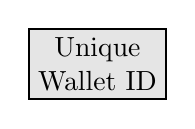
\begin{tikzpicture}
        \node [fill=gray!20,draw=black,thick,align=center] { Unique \\ Wallet ID};
      \end{tikzpicture}
    }}
    \newinst[2]{exchange}{\shortstack{Taler (exchange) \\
       \\ \begin{tikzpicture}[shape aspect=.5]
        \tikzset{every node/.style={cylinder,shape border rotate=90, draw,fill=gray!25}}
        \node at (1.5,0) {\shortstack{{{\tiny Database}}}};
       \end{tikzpicture}
    }}
    \newinst[2]{sms}{\shortstack{Address validator}}

    \postlevel
    \mess[0]{wallet}{{P2P payment (Wallet ID)}}{exchange}
    \begin{callself}{exchange}{New wallet?}{}
    \end{callself}
    \mess[0]{exchange}{Request address validation}{sms}
    \mess[0]{sms}{Validation process ID}{exchange}
    \mess[0]{exchange}{Request address validation}{wallet}
    \mess[0]{wallet}{Send address}{sms}
    \mess[0]{sms}{{Send confirmation code (to address)}}{wallet}
    \mess[0]{wallet}{Supply confirmation code}{sms}
    \mess[0]{sms}{{Confirmed customer address}}{exchange}
    \mess[0]{exchange}{{Confirm completion}}{wallet}
    \mess[0]{wallet}{{Retry action}}{exchange}
\end{sequencediagram}
  \caption{Deposit interactions between customer, Taler exchange (payment
    service provider) and external address validation service.  The process can be
    triggered by wallet-to-wallet (P2P) payments described in Chapter~\ref{chap:triggers}.}
  \label{fig:proc:domestic}
\end{figure}

Our users have to accept the terms of service which restrict the use of the
service to domestic customers.  For interactions with the core banking system,
this simply means that we only accept payments from or to domestic bank
accounts.  For P2P payments between wallets, we require that the wallets are
controlled by a domestic entity.  We define domestic entities as those that
are able to receive messages at a domestic address. Two types of addresses are
supported:

\begin{itemize}
\item Control over a domestic {\bf mobile phone number} is established
  by sending an SMS message with a confirmation code to the MSIN.
\item Control over a domestic {\bf postal address} is established by
  sending a letter with a confirmation code to the address.
\end{itemize}

Depending on the type of address, a validation has a limited validity period,
as shown in Table~\ref{table:proc:domestic}.  When the validity period is
over, a wallet has to re-do the address validation before they can receive any
further funds through the service.

\begin{table}[h!]
  \caption{Restrictions on address validations}
  \label{table:proc:domestic}
  \begin{tabular}{l|l|r}
    {\bf Type}          & {\bf Validity period} & {\bf Restricted to} \\ \hline \hline
    Mobile phone number & 12 months             & {\em +41} \\
    Postal address      & 36 months             & {\em Switzerland} \\
  \end{tabular}
\end{table}
